\chapter{Technology Review}
\label{chap:technology_review}

\section{Overview of Patented Climbing Wall Technologies}

The US Patent US5919117A entitled: 'Climbing Training Apparatus' \cite{US5919117A} describes the device as being “a movable climbing training wall surface defined by a continuous belt rotatably disposed about a pivotable frame and controllably actuated to rotate at a selected speed”.\\
The patent was filed on 1999-07-06 and subsequently expired on 2017-01-29. It is now classified as Expired - Fee Related.\\\\
A similar patent US005125877A entitled: 'Simulated Climbing Wall' \cite{US5125877A} also describes a rotating climbing device. This patent is also expired.\\\\
There is thus currently no commercial restriction on rotating climbing apparatus and simulated climbing walls and this project is therefore able to proceed with development of a rotary climbing wall.

\section{Analysis of Current Climbing Wall Models}
The rotating climbing wall market currently offers a range of products, from higher-end systems equipped with extensive features as well as more economic systems with fewer functionality. \\\\
After evaluating the current systems available, the list below outlines the main functions currently available on the market:

\begin{itemize}
    \item Adjustable Speed
    \item Adjustable Incline
    \item Automatic pause/continue rotation
    \item Can operate without electricity
    \item Monitor Results
    \item  Terrain Editor
    \item Automatic Climbing modes/difficulty
\end{itemize}

\subsection{Xclimbpro Rotating Climbing Wall} (\url{https://xclimbpro.com/})
\begin{figure}[H]
    \centering
    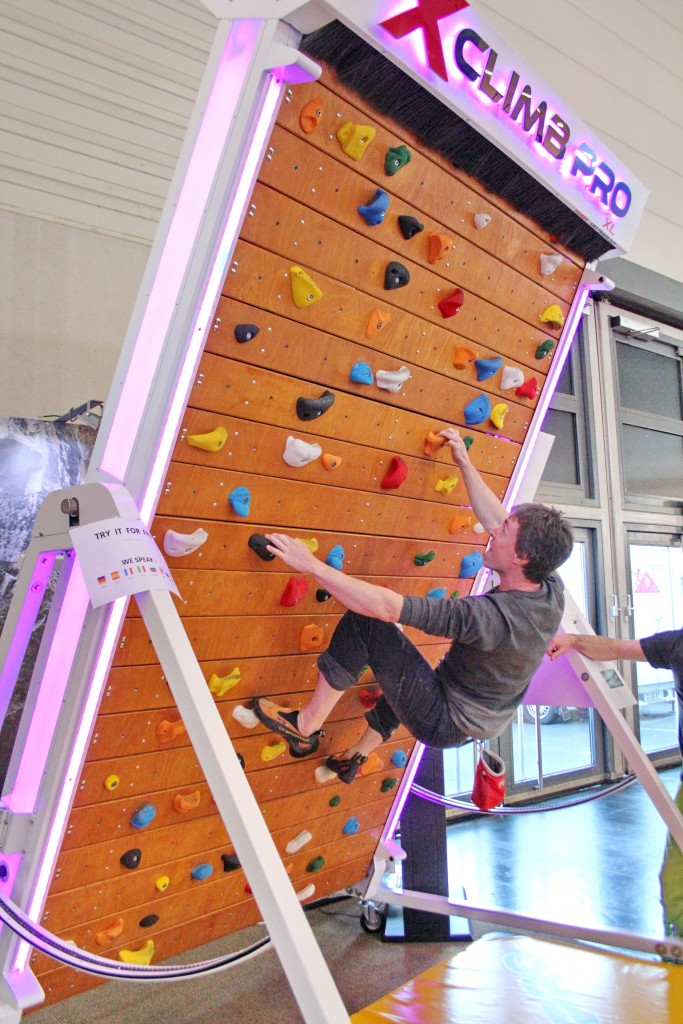
\includegraphics[width=0.6\linewidth]{figs/Xclimbpro.jpg}
    \caption{Xclimbpro Rotating Climbing Wall}
\end{figure}
    \begin{itemize}
        \item Features adjustable speed and can operate without electricity, offering an optional 12V adapter.
        \item Offers versatility in installation, being wall-mountable or movable with optional casters.
        \item Models include:
        \begin{itemize}
            \item Model S: Compact and budget-friendly.
            \item Model M: Features increased width and angle adjustment from +35° to -35°.
            \item Model L: Offers larger dimensions for all skill levels.
            \item Model XL: Stands 3.5m tall, accommodating 2-3m climbers with a -35° inclination.
        \end{itemize}
    \end{itemize}

\subsection{Climbstation Climbing Wall}
(\url{https://www.climbstation.com/})
\begin{figure}[H]
    \centering
    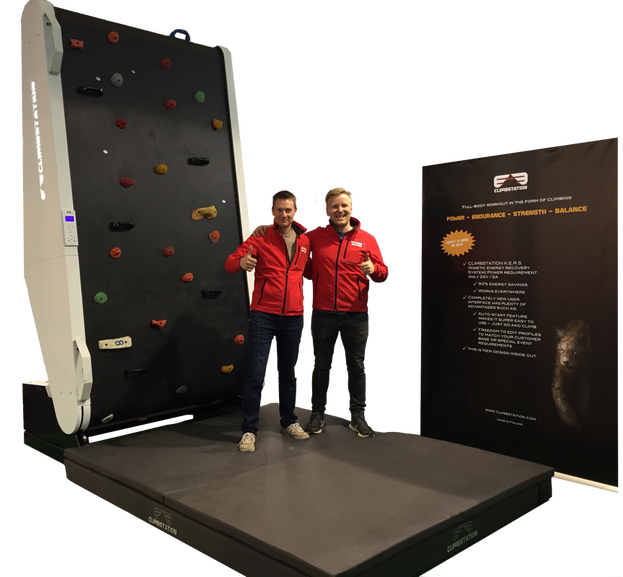
\includegraphics[width=0.9\linewidth]{figs/climbstation.png}
    \caption{Climbstation Climbing Wall}
\end{figure}
    \begin{itemize}
        \item The operational size is 330 cm in height by 190 cm in width and 380 cm in length.
        \item Allows for adjustable climbing surface angles from +15° to -45°.
        \item Achieves the highest climbing speed of 25 meters per minute.
        \item Includes 70 standard handholds, 
        \item Powered by a 24-30V / 2A / 50-60Hz source.
        \item Key functions and features include Terrain Editor, Restore Function, Climb Data and Payment System Support, Unlimited Climbing Options, and Monitoring of Results.
    \end{itemize}

\subsection{TreadWall}
(\url{https://treadwallfitness.com/})
\begin{figure}[H]
    \centering
    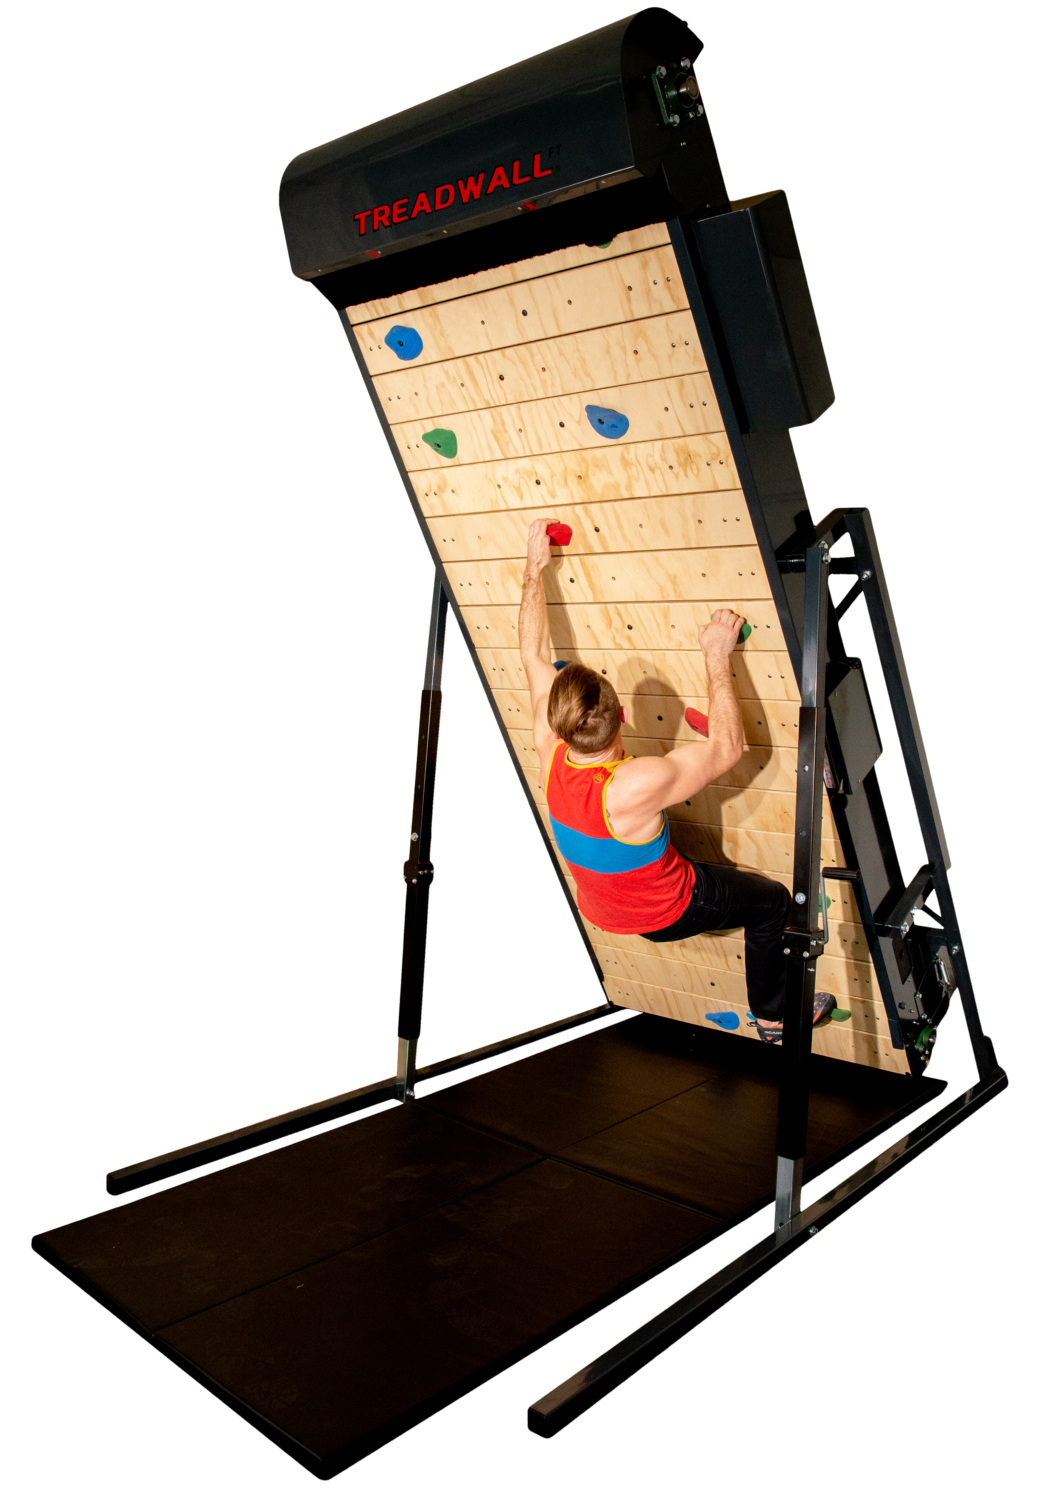
\includegraphics[width=0.5\linewidth]{figs/treadwall_kore4.png}
    \caption{Treadwall Kore4}
\end{figure}
    \begin{itemize}
        \item Features adjustable speed and some models can operate without electricity.
        \item Features adjustable inclination, with certain models adjusting this automatically and others manually.
        \item Automatically pauses when climber's weight on bottom rung.
        \item 180 possible hold placements
        \item Features electronic display that measures speed, distance,  time, and calories.
        \item Models include:
        \begin{itemize}
            \item V4: Base model without incline ability.
            \item Kore4: Budget model for home use. Features incline ability.
            \item S4: Larger model for gym use. All features available.
            \item Max6: Flagship model with a 3.1m height and 1.83m width. All features available
        \end{itemize}
        
    \end{itemize}

\section{Detailed Product Comparisons}
The table below provides a comprehensive summary of the functionalities available in each product.

\begin{table}[H]
\centering
\caption{Comparison of Climbing Wall Models}
\label{tab:climbing_wall_comparison}
\resizebox{\textwidth}{!}{%
\begin{tabular}{|p{0.12\linewidth}|p{0.08\linewidth}|p{0.08\linewidth}|p{0.1\linewidth}|p{0.1\linewidth}|p{0.1\linewidth}|p{0.12\linewidth}|p{0.2\linewidth}|p{0.1\linewidth}|}
\hline
System & Width [m] & Height [m] & Incline & Adjust\newline Speed & Monitor & Extra\newline Functions & Construction\newline Material & Price \\
\hline
XClimb\newline Pro S & 1.5 & 2.82 & No & Yes & No & No & Steel/Wood & R230000 \\
\hline
XClimb\newline Pro XL & 2 & 3.48 & Auto& Yes & No & No & Steel/Wood & R278000 \\
\hline
Climb\newline Station & 1.9 & 3.3 & Auto& Auto & Yes & Advanced Control\newline Panel & Aluminium & N/A \\
\hline
Treadwall V4 & 1.22 & 2.97 & No & Manual & Yes & auto-stop & Steel/Wood & R202000 \\
\hline
Treadwall Kore4/11 & 1.22 & 2.75 & Manual & Manual & Yes & auto-stop & Steel/Wood & R140600 \\
\hline
Treadwall S4/12 & 1.22 & 3.1 & Manual & Manual & Yes & auto-stop & Steel/Wood & R218000 \\
\hline
Treadwall Max6/12 & 1.83 & 3.1 & Manual & Manual & Yes & auto-stop & Steel/Wood & R227200 \\
\hline
\end{tabular}
}
\end{table}

\section{Selection of Features for Proposed Climbing Wall Design}
In order to effectively train the three core physiological pillars of climbing—strength, power, and endurance—the design of the rotary training device must feature adjustable speed and inclination. While additional functionalities such as automatic adjustments for speed and inclination during use, along with metrics for tracking distance climbed and calories burned, may enhance usability, they are not essential for this prototype.\\\\
From the analysis presented in Table \ref{tab:climbing_wall_comparison}, as well as general design overview, a few unique concepts for each sub-system were derived.



